\documentclass[tikz,border=10pt]{standalone}
\usepackage{tikz}
\usetikzlibrary{shapes.geometric, arrows.meta, positioning, calc, fit, backgrounds}
\usepackage{amsmath,amssymb}
\usepackage{xcolor}

% Unified Academic Color Palette
\definecolor{cInput}{RGB}{235, 248, 255}
\definecolor{bInput}{RGB}{49, 130, 206}

\definecolor{cTrans}{RGB}{240, 249, 255}
\definecolor{bTrans}{RGB}{43, 108, 176}

\definecolor{cGCN}{RGB}{230, 255, 250}
\definecolor{bGCN}{RGB}{49, 151, 149}

\definecolor{cRecurr}{RGB}{250, 245, 255}
\definecolor{bRecurr}{RGB}{128, 90, 213}

\definecolor{cHead}{RGB}{255, 245, 245}
\definecolor{bHead}{RGB}{229, 62, 62}

\definecolor{cFusion}{RGB}{254, 252, 191}
\definecolor{bFusion}{RGB}{214, 158, 46}

\definecolor{cGray}{RGB}{247, 250, 252}
\definecolor{bGray}{RGB}{160, 174, 192}

\definecolor{tDark}{RGB}{26, 32, 44}
\definecolor{tMuted}{RGB}{74, 85, 104}

\begin{document}
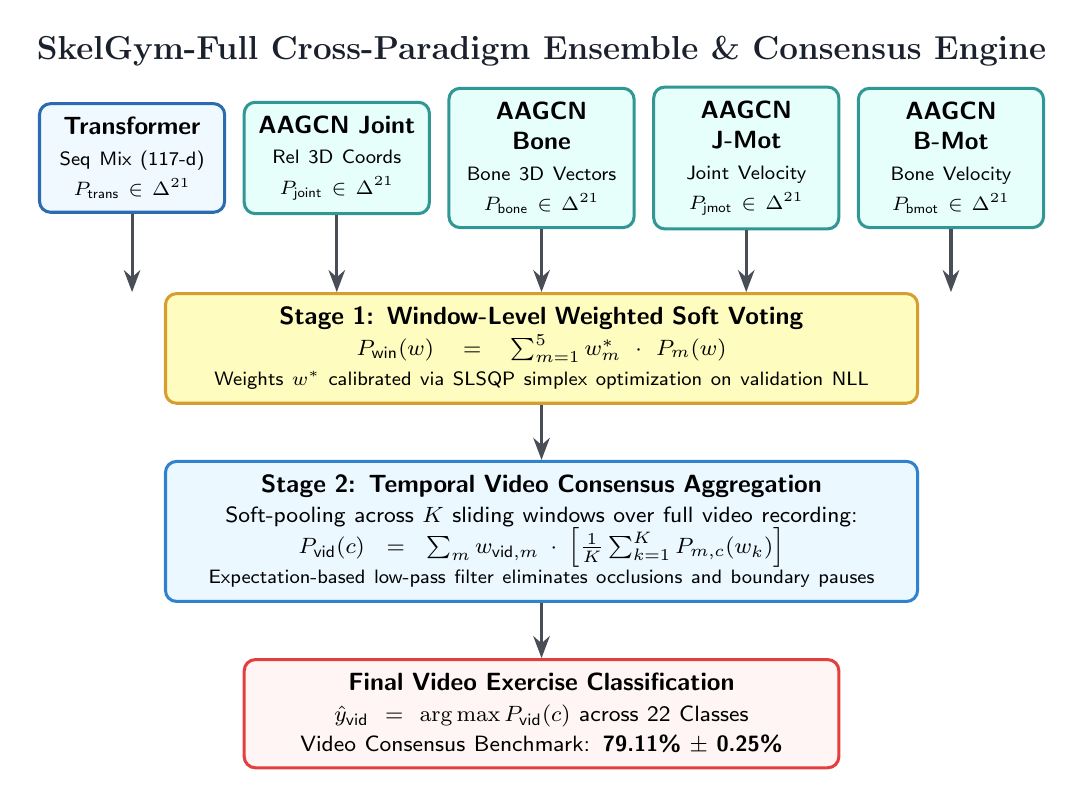
\begin{tikzpicture}[
    font=\sffamily\small,
    >=Stealth,
    node distance=0.6cm,
    block/.style={
        draw=#1,
        line width=1.1pt,
        rounded corners=4pt,
        align=center,
        inner sep=5pt
    },
    arrow/.style={->, line width=1.1pt, color=tDark!80}
]

\node[font=\bfseries\large, text=tDark] (title) at (6.0, 1.35) {SkelGym-Full Cross-Paradigm Ensemble \& Consensus Engine};

\node[block=bTrans, fill=cTrans, text width=2.0cm] (e1) at (0.8, 0) {
    \textbf{Transformer}\\
    {\scriptsize Seq Mix (117-d)}\\
    {\scriptsize $P_{\text{trans}} \in \Delta^{21}$}
};
\node[block=bGCN, fill=cGCN, text width=2.0cm] (e2) at (3.4, 0) {
    \textbf{AAGCN Joint}\\
    {\scriptsize Rel 3D Coords}\\
    {\scriptsize $P_{\text{joint}} \in \Delta^{21}$}
};
\node[block=bGCN, fill=cGCN, text width=2.0cm] (e3) at (6.0, 0) {
    \textbf{AAGCN Bone}\\
    {\scriptsize Bone 3D Vectors}\\
    {\scriptsize $P_{\text{bone}} \in \Delta^{21}$}
};
\node[block=bGCN, fill=cGCN, text width=2.0cm] (e4) at (8.6, 0) {
    \textbf{AAGCN J-Mot}\\
    {\scriptsize Joint Velocity}\\
    {\scriptsize $P_{\text{jmot}} \in \Delta^{21}$}
};
\node[block=bGCN, fill=cGCN, text width=2.0cm] (e5) at (11.2, 0) {
    \textbf{AAGCN B-Mot}\\
    {\scriptsize Bone Velocity}\\
    {\scriptsize $P_{\text{bmot}} \in \Delta^{21}$}
};

% Stage 1: Window-Level Weighted Soft Voting
\node[block=bFusion, fill=cFusion, text width=9.2cm, below=0.8cm of e3] (s1) {
    \textbf{Stage 1: Window-Level Weighted Soft Voting}\\
    {\footnotesize $P_{\text{win}}(w) = \sum_{m=1}^5 w_m^* \cdot P_m(w)$}\\
    {\scriptsize Weights $w^*$ calibrated via SLSQP simplex optimization on validation NLL}
};

\draw[arrow] (e1.south) -- (s1.north -| e1.south);
\draw[arrow] (e2.south) -- (s1.north -| e2.south);
\draw[arrow] (e3) -- (s1);
\draw[arrow] (e4.south) -- (s1.north -| e4.south);
\draw[arrow] (e5.south) -- (s1.north -| e5.south);

% Stage 2: Temporal Video Consensus Aggregation
\node[block=bInput, fill=cInput, text width=9.2cm, below=0.7cm of s1] (s2) {
    \textbf{Stage 2: Temporal Video Consensus Aggregation}\\
    {\footnotesize Soft-pooling across $K$ sliding windows over full video recording:}\\
    {\footnotesize $P_{\text{vid}}(c) = \sum_{m} w_{\text{vid}, m} \cdot \left[ \frac{1}{K} \sum_{k=1}^K P_{m, c}(w_k) \right]$}\\
    {\scriptsize Expectation-based low-pass filter eliminates occlusions and boundary pauses}
};

\draw[arrow] (s1) -- (s2);

% Final Output
\node[block=bHead, fill=cHead, text width=7.2cm, below=0.7cm of s2] (pred) {
    \textbf{Final Video Exercise Classification}\\
    {\footnotesize $\hat{y}_{\text{vid}} = \arg\max P_{\text{vid}}(c)$ across 22 Classes}\\
    {\footnotesize Video Consensus Benchmark: \textbf{79.11\% $\pm$ 0.25\%}}
};

\draw[arrow] (s2) -- (pred);

\end{tikzpicture}
\end{document}
